\begin{center}
    \Large{\textbf{Теоретична частина}}    
\end{center}

\vspace{1mm}

У цій роботі вивчається інтерференційна картина,
що виникає при освітленні єдиним світловим пучком
товстої плоскопаралельної скляної пластини, тобто використовується 
метод поділу амплітуди. В цьому випадку світлові промені, 
що інтерферують формуються при відбиванні світла від граней пластини 
(див.рис.1).

\begin{wrapfigure}{l}{0.5\textwidth}    
    \centering
    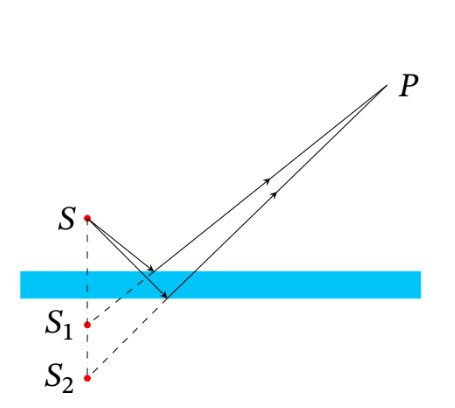
\includegraphics[width=.4\textwidth]{assets/separate_amplitude.png}
    \caption{Схема інтерференції методом поділу амплітуди}
\end{wrapfigure}

У будь-яку точку $P$, що знаходиться з тієї 
ж сторони від пластинки, що і джерело, приходять
два променя (при малому коефіцієнті відбиття 
та при малих кутах падіння, повторні відбивання
від внутрішніх поверхонь пластинки можна не брати до уваги,
оскільки енергія пучків, що зазнали двох та більшого
числа відбивань дуже мала). Ці промені утворюють інтерференційну картину.
Для визначення вигляду смуг можна уявити собі, що промені виходять з уявних
зображень $S_1$ і $S_2$ реального джерела $S$. На віддаленому екрані,
розташованому паралельно пластині, інтерференційні смуги мають вигляд концентричних
кілець, центр яких знаходиться на осі, що перпендикулярна до пластини і
проходить через джерело $S$.


В роботі використовується варіант побудови оптичної схеми, де пластина
освітлюється світловим пучком від точкового джерела 
(яке моделюється фокусом лінзи, що освітлюється лазером, рис. 2).
Для опису інтерференційної картини необхідно визначити,
які промені сходяться в кожній точці екрану і яка оптична різниця ходу між ними.
На рис. 2 показаний хід двох інтерферуючих променів, що приходять
в точку спостереження $P$. Для того, щоб промені зійшлися в одній точці, має
виконуватися умова:

\begin{equation} \label{eq:1}
    d \tan{\beta} = L(\tan{(i+ \delta i)} - \tan{i})
\end{equation}

Оскільки кути дуже малі, то ми можемо скористатись наближеними 
формулами $\tan{i} \simeq i $, Прості тригонометричні перетворення з урахуванням закону 
заломлення світла ($ \frac{i}{b} = n $) призводять до наступного виразу для різниці кутів
падіння цих променів:

\begin{equation} \label{eq:2}
    \delta i = \frac{d}{nL}i
\end{equation}

Оптична різниця ходу між цими променями:

\begin{equation} \label{eq:3}
    \Delta = 2(SR + n RM - SQ ) - \frac{\lambda}{2} = \\
    2 \left( \frac{nd}{\cos{\beta}} + \frac{L}{\cos{i}} - \frac{L}{\cos{(i + \delta i)}} \right) - \frac{\lambda}{2}
\end{equation}

\begin{figure}[h]
    \centering    
    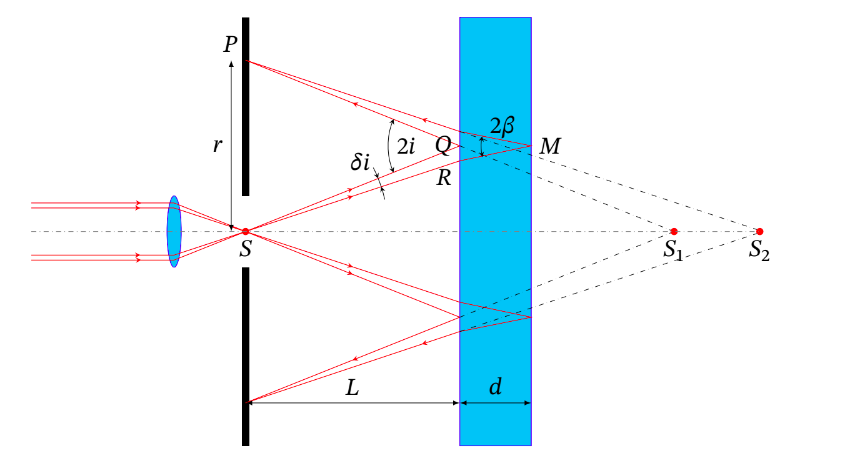
\includegraphics[width=.5\textwidth]{assets/main_scheme.png}       
    \caption{Схема дослідної установки}
\end{figure}

Останній доданок $\frac{\lambda}{2}$
враховує зміну фази хвилі при відбиванні від середовища
з більш високим показником заломлення («втрата напівхвилі»).

При використанні наближених виразів для функцій малих кутів(
$i \simeq \frac{r}{2L}, 
\frac{i}{\cos{i}} \simeq 1 + \frac{i^2}{2},
\beta = \frac{i}{n}, \frac{1}{\beta} = 1 + \frac{i^2}{2n^2} $)
співвідношення \ref{eq:3} зводиться до:

\begin{equation} \label{eq:4}
    \Delta = 2nd - \frac{d}{b} \frac{r^2}{4L^2} - \frac{\lambda}{2}
\end{equation}

З отриманого співвідношення видно, по-перше,
що різниця ходу залежить тільки від кута $i$
(кут заломлення $\beta$ пов’язаний з кутом падіння
i законом Снеліуса $\sin{i} = n \sin{\beta}$). Отже,
вона буде однаковою для всіх точок екрану з
однаковим i, тобто для кіл з центром в точці $S$.
Це означає, що інтерференційна картина повинна складатися з концентричних кілець.


По-друге, зі співвідношення \ref{eq:2} видно, що
$\delta i \ll i$, тобто, інтерферуючі промені

мають практично рівні кути падіння на пластину,
рівні нахили. Тому смуги, що спостерігаються
на інтерференційній картині називаються смугами рівного нахилу.


Найбільшою оптична різниця ходу при нормальному падінні променів
($i = 0, r = 0$) і дорівнює $\Delta_{max} = 2nd - \frac{\lambda}{2}$.
Далі вона монотонно спадає з ростом $r$.


Мінімуми інтерференційної картини спостерігаються при таких значеннях
$r$ при яких оптична довжина ходу стає рівною:

\begin{equation} \label{eq:5}
    \Delta = \left( m - \frac{1}{2} \right) \lambda
\end{equation}

де ціле число $m \in \mathbb{Z}$ – порядок інтерференції. Причому, слід зазначити,
що порядок інтерференції зростає від периферії екрану до його центру. Для
зручності, краще перенумерувати порядки інтерференції від центру до периферії,
такі числа будемо позначати як $k$.
Прирівняємо формули \ref{eq:4} та \ref{eq:5} і (врахувавши нову нумерацію)
отримаємо вираз:

$$ 2nd - \frac{d}{n} \frac{r^2}{4L^2} = k \lambda $$


Запишемо цю формулу для двох темних кілець з номерами $m_1, m_2$:

$$
\begin{cases} 
    2nd - \frac{d}{n} \frac{r_1^2}{4L^2} = k_1 \lambda \\[1em]
    2nd - \frac{d}{n} \frac{r_2^2}{4L^2} = k_2 \lambda
\end{cases}
$$

Віднявши від другого рівняння системи перше виразимо звідси:

$$ \frac{r_2^2 - r_1^2}{k_2 - k_1} = \frac{4nL^2 \lambda}{d} $$

Оскільки $ k_2 - k_1 = \Delta N \in \mathbb{Z} $,
то останню формулу можна переписати у вигляді:

\begin{equation} \label{eq:6}
    \frac{\Delta r^2}{\Delta N} = \frac{4nL^2 \lambda}{d}
\end{equation}

Отже, побудувавши графік залежності 
$r^2 = f(N)$, можна визначити при фіксованому L
будь-яку з величин $\lambda, n$ або $d$, якщо відомі дві інші.


\begin{figure}[h]
    \centering    
    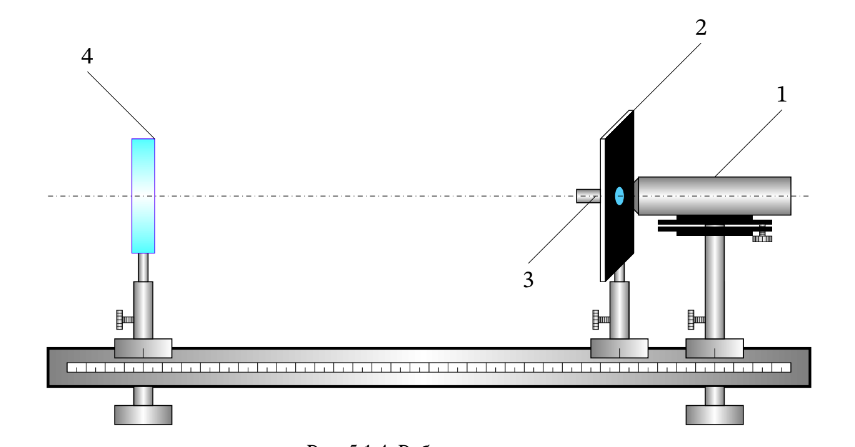
\includegraphics[width=.6\textwidth]{assets/experiment_tools.png}
    \caption{Схема дослідної установки}
\end{figure}

Схема установки показані на рис. 3. До складу установки входять:
лазер 1, короткофокусна оптична система 3 з екраном спостереження 2,
скляна плоскопаралельна пластина 4. Ці вузли установки закріплені
в рейтерах, встановлених на металеву основу. Пучок лазера падає
на збиральну лінзу 3, на оправі якої закріплений екран спостереження
таким чином, що фокальна площинулінзи поєднана з площиною цього екрану. 
Екран спостереження має отвір для
проходження світлового пучка. Сфокусований лінзою світловий пучок можна
розглядати як точковий джерело світлової хвилі зі сферичним хвильовим фронтом.
Цей пучок падає на непаралельну пластину, встановлену перпендикулярно
осі пучка. Основна частина пучка проходить через пластину і затримується
захисним екраном. світлові пучки, відбиті в зворотному напрямку від передньої
і задньої граней пластини, потрапляють на екран спостереження, утворюючи на
ньому інтерференційну картину концентричних темних і світлих кілець. Слід
зазначити, що симетрія інтерференційної картини визначається симетрією ходу
променів в установці. В даному випадку це осьова симетрія пучка лазера і 
сферичної лінзи. На поверхню екрана нанесена міліметрова шкала для вимірювання
розмірів інтерференційної картини.

%\begin{figure}[h]    
%    \centering
%    \includegraphics[width=.7\textwidth]{assets/filename }
%    \caption{Підпис}
%\end{figure}